\section{Introduction}













\begin{wrapfigure}[21]{r}{0.4\textwidth}  %
  \centering
    \vspace{-1.5em}
    \includegraphics[width=\linewidth]{figures/main/intro_scaling_cropped.pdf}
	\caption{\small{Sample quality vs. effective sampling compute (billion parameters $\times$ number of function evaluations during sampling). We compare the sample quality of different models on ImageNet 512$\times$512, measured by FID ($\downarrow$). Our 2-step sCM achieves sample quality comparable to the best previous generative models while using less than 10\% of the effective sampling compute.}
	\label{fig:intro_scaling}}
    \vspace{-0.5em}
\end{wrapfigure}


Diffusion models~\citep{sohl2015deep,song2019generative,ho2020ddpm,song2020score} have revolutionized generative AI, achieving remarkable results in image~\citep{rombach2022high,ramesh2022hierarchical,ho2022imagen}, 3D~\citep{poole2022dreamfusion,wang2024prolificdreamer,liu2023zero}, audio~\citep{liu2023audioldm,evans2024fast}, and video generation~\citep{blattmann2023stable,videoworldsimulators2024}. Despite their success, a significant drawback is their slow sampling speed, often requiring dozens to hundreds of steps to generate a single sample. Various diffusion distillation techniques have been proposed, including direct distillation~\citep{luhman2021knowledge,zheng2023dfno}, adversarial distillation~\citep{wang2022diffusion-stylegan,sauer2023adversarial}, progressive distillation~\citep{salimans2022progressive}, and variational score distillation (VSD)~\citep{wang2024prolificdreamer,yin2024dmd,yin2024dmd2,luo2024diff-instruct,xie2024EMD,salimans2024multistepmoment}. However, these methods come with challenges: direct distillation incurs extensive computational cost due to the need for numerous diffusion model samples; adversarial distillation introduces complexities associated with GAN training; progressive distillation requires multiple training stages and is less effective for one or two-step generation; and VSD can produce overly smooth samples with limited diversity and struggles at high guidance levels.

Consistency models (CMs)~\citep{song2023cm,song2023ict} offer significant advantages in addressing these issues. They eliminate the need for supervision from diffusion model samples, avoiding the computational cost of generating synthetic datasets. CMs also bypass adversarial training, sidestepping its inherent difficulties. Aside from distillation, CMs can be trained from scratch with consistency training (CT), without relying on pre-trained diffusion models. Previous work~\citep{song2023ict,geng2024ect,luo2023latent,xie2024mlcm} has demonstrated the effectiveness of CMs in few-step generation, especially in one or two steps. However, these results are all based on discrete-time CMs, which introduces discretization errors and requires careful scheduling of the timestep grid, potentially leading to suboptimal sample quality. In contrast, continuous-time CMs avoid these issues but have faced challenges with training instability~\citep{song2023cm,song2023ict,geng2024ect}.


\begin{figure}[t]
\centering
	\begin{minipage}{0.3\linewidth}
		\centering
			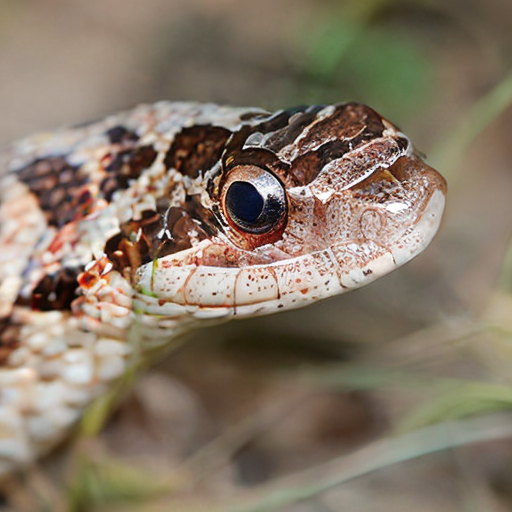
\includegraphics[width=\linewidth]{figures/samples-intro/54.png}\\
			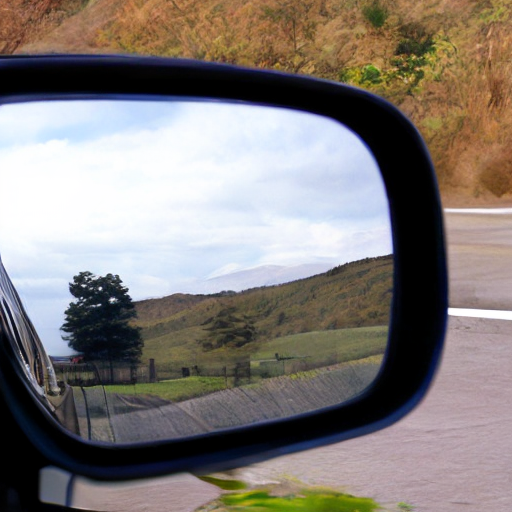
\includegraphics[width=\linewidth]{figures/samples-intro/475.png}\\
			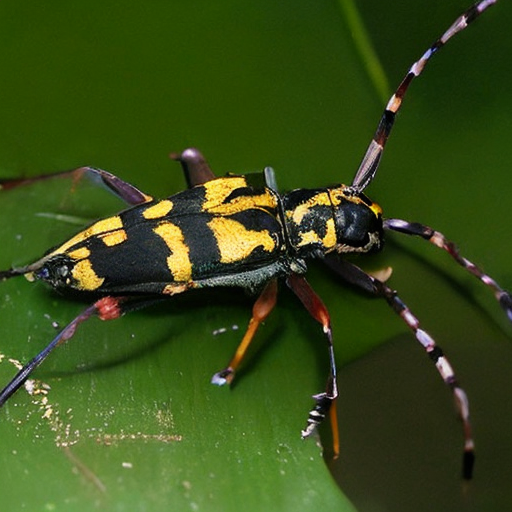
\includegraphics[width=\linewidth]{figures/samples-intro/303.png}\\
	\end{minipage}
	\begin{minipage}{0.3\linewidth}
		\centering
			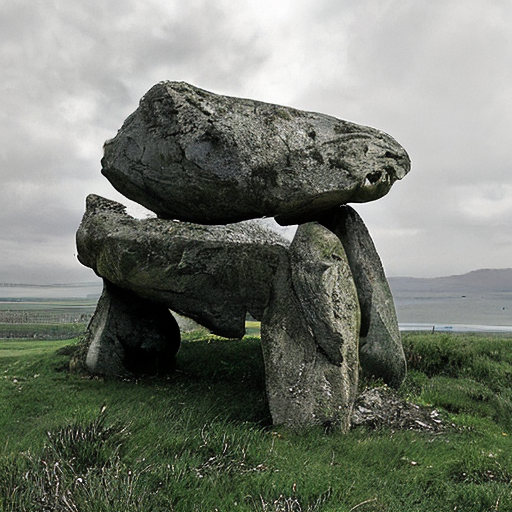
\includegraphics[width=\linewidth]{figures/samples-intro/649.png}\\
			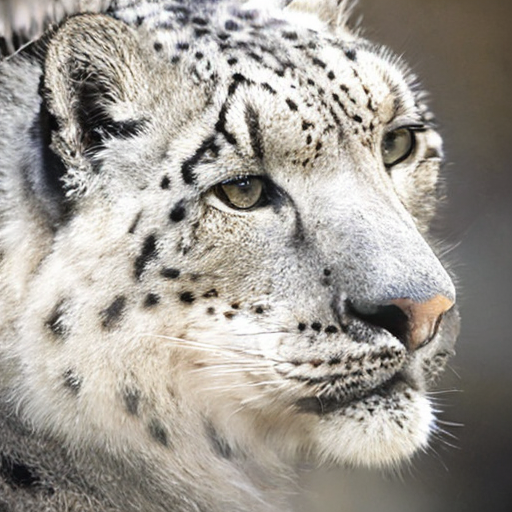
\includegraphics[width=\linewidth]{figures/samples-intro/289.png}\\
			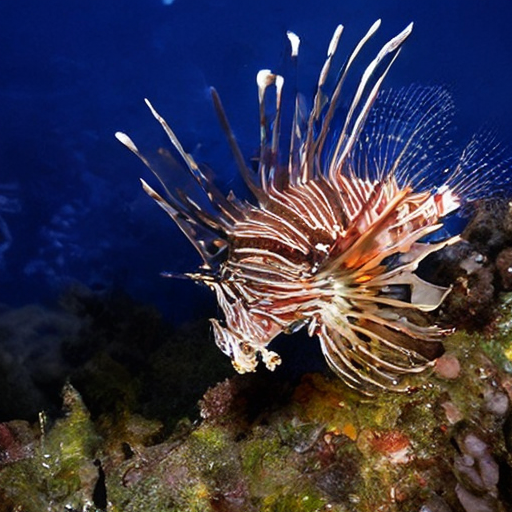
\includegraphics[width=\linewidth]{figures/samples-intro/396.png}\\
	\end{minipage}
	\begin{minipage}{0.3\linewidth}
		\centering
			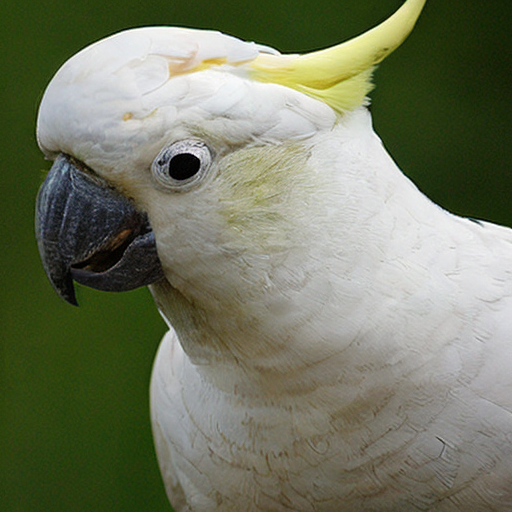
\includegraphics[width=\linewidth]{figures/samples-intro/89.png}\\
			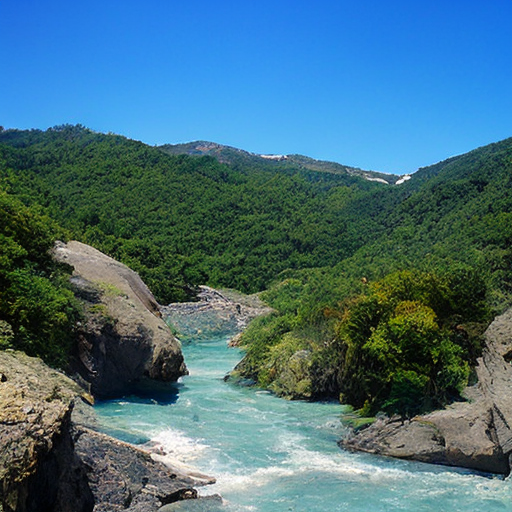
\includegraphics[width=\linewidth]{figures/samples-intro/979.png}\\
			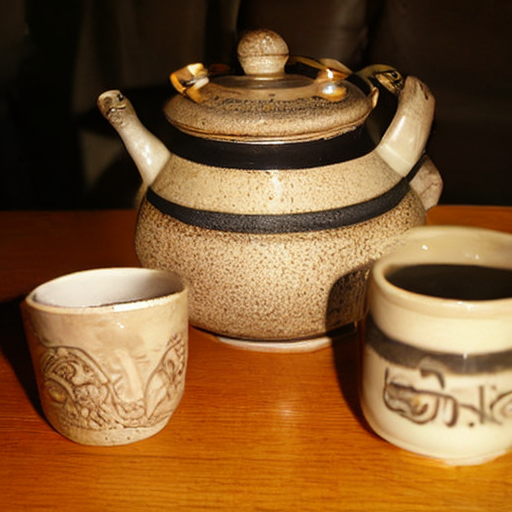
\includegraphics[width=\linewidth]{figures/samples-intro/849.png}\\
	\end{minipage}
	\caption{\small{Selected 2-step samples from a continuous-time consistency model trained on ImageNet 512$\times$512.}
	\label{fig:intro:samples}}
\vspace{-.2in}
\end{figure}


In this work, we introduce techniques to simplify, stabilize, and scale up the training of continuous-time CMs. Our first contribution is TrigFlow, a new formulation that unifies EDM~\citep{karras2022edm,karras2024edm2} and Flow Matching~\citep{peluchetti2022nondenoising,lipman2022flowmatching,rectified_flow,albergo2023stochastic_interpolants,heitz2023iterative}, significantly simplifying the formulation of diffusion models, the associated probability flow ODE and CMs. Building on this foundation, we analyze the root causes of instability in CM training and propose a complete recipe for mitigation. Our approach includes improved time-conditioning and adaptive group normalization within the network architecture. Additionally, we re-formulate the training objective for continuous-time CMs, incorporating adaptive weighting and normalization of key terms, and progressive annealing for stable and scalable training. 

With these improvements, we elevate the performance of consistency models in both consistency training and distillation, achieving comparable or better results compared to previous discrete-time formulations. Our models, referred to as sCMs, demonstrate success across various datasets and model sizes. We train sCMs on CIFAR-10, ImageNet 64$\times$64, and ImageNet 512$\times$512, reaching an unprecedented scale with 1.5 billion parameters---the largest CMs trained to date (samples in \figref{fig:intro:samples}). We show that sCMs scale effectively with increased compute, achieving better sample quality in a predictable way. Moreover, when measured against state-of-the-art diffusion models, which require significantly more sampling compute, sCMs narrow the FID gap to within 10\% using two-step generation. In addition, we provide a rigorous justification for the advantages of continuous-time CMs over discrete-time variants by demonstrating that sample quality improves as the gap between adjacent timesteps narrows to approach the continuous-time limit. Furthermore, we examine the differences between sCMs and VSD, finding that sCMs produce more diverse samples and are more compatible with guidance, whereas VSD tends to struggle at higher guidance levels.
